\chapter{Applications of Differentiation}
\label{chappdiff}

The derivative of a function describes how the values of a function change,
and this indication of change can be used to understand a function better or
to find $x$-values at which the function behaves in a particular way (such
as having maxima, minima, or zeroes).

One way to think about this is if you imagine the graph of a function to
depict the track (viewed from above) along which a bicycle rode.
There are places where the rider performed actions to change the way she
rode, and other places where she basically continued in the same way as
before. These are the places we want to identify.

In many textbooks this topic goes under the name of ``curve sketching'',
which was a main application before the advent of easily accessible plotting
tools. However, even if we do not want to plot a function by hand,
understanding how a function and its derivatives are related is useful for
applications.

\section{Increasing and Decreasing}
\label{secincr}

The value of the derivative is the slope of the tangent line to the graph.
That means that the graph goes up
when the derivative is positive and goes down
when the derivative is negative. More formally, using the same language as
with sequences:
\begin{defn}
Let $D\subset\R$ and $f\colon D\to\R$ a differentiable function and $x_0\in
D$. We say that $f$ is
\begin{description}
\item[\defini{increasing} at $x_0$] if $f(x_0)\ge 0$.
\item[\defini{strictly increasing} at $x_0$] if $f(x_0)\gneqq 0$.
\item[\defini{decreasing} at $x_0$] if $f(x_0)\le 0$.
\item[\defini{strictly decreasing} at $x_0$] if $f(x_0)\lneqq 0$.
\end{description}
We say that $f$ is increasing (\& c.) on $D$, if it its increasing
(\& c.) at every $x_0\in D$
\end{defn}
Note that $f$ is increasing on $D$ if $f(a)\ge f(b)$ (strictly, if
$f(a)\gneqq f(b)$) whenever $a>b$. We have analogous definitions for
decreasing. (and

This allows us to characterize when differentiable functions are one-to-one:
A function that is strictly increasing must be one-to-one, since two
different points in the domain must have one of them larger ($a$, say), and
then $f(a)>f(b)$, in particular $f(a)\not=f(b)$.

Again the same holds for a strictly decreasing function. We also see easily
that a (continuous) function that first increases and then decreases must
reach the same value twice, and thus cannot be one-to-one.

The only further
case that is permitted is if $f'(x_0)=0$ at individual points (as for $x^3$ at
$x=0$). We state this (without a formal proof, that would be somewhat
technical):
\begin{lemma}
Let $f\colon D\to\R$ be a differentiable function. Then $f$ is one-to one, if
and only if $f$ is increasing on $D$ (or decreasing on $D$), and strictly
increasing (respectively strictly decreasing) at all but finitely many
points in $D$.
\end{lemma}

\section{The Shape of a Curve}
\label{secshape}

Knowing where a function increases and decreases also helps us to describe
the overall shape of the graph of a function. Consider for example the
graph\mynote{In case someone cares, it is the horribly looking horribly
looking  function
$1109/31850496x^9-63797/79626240x^8+114341/19906560x^7-61627/9953280x^6-823919/9953280x^5+1137739/4976640x^4+68581/207360x^3-5731/4320x^2+2$}
of a function $f\colon\R\to\R$ in Figure~\ref{figkurvdiss1}:
\begin{figure}
\begin{center}
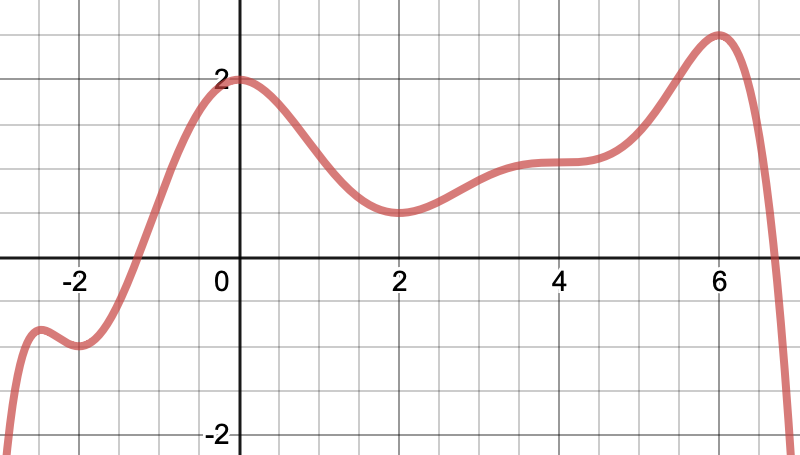
\includegraphics[width=8cm]{pic/kurvdiss1.png}
\end{center}
\caption{The graph of a function}
\label{figkurvdiss1}
\end{figure}

We calculate the derivative and look at where the derivative is negative
(that is the original function is decreasing):
\begin{figure}
\begin{center}
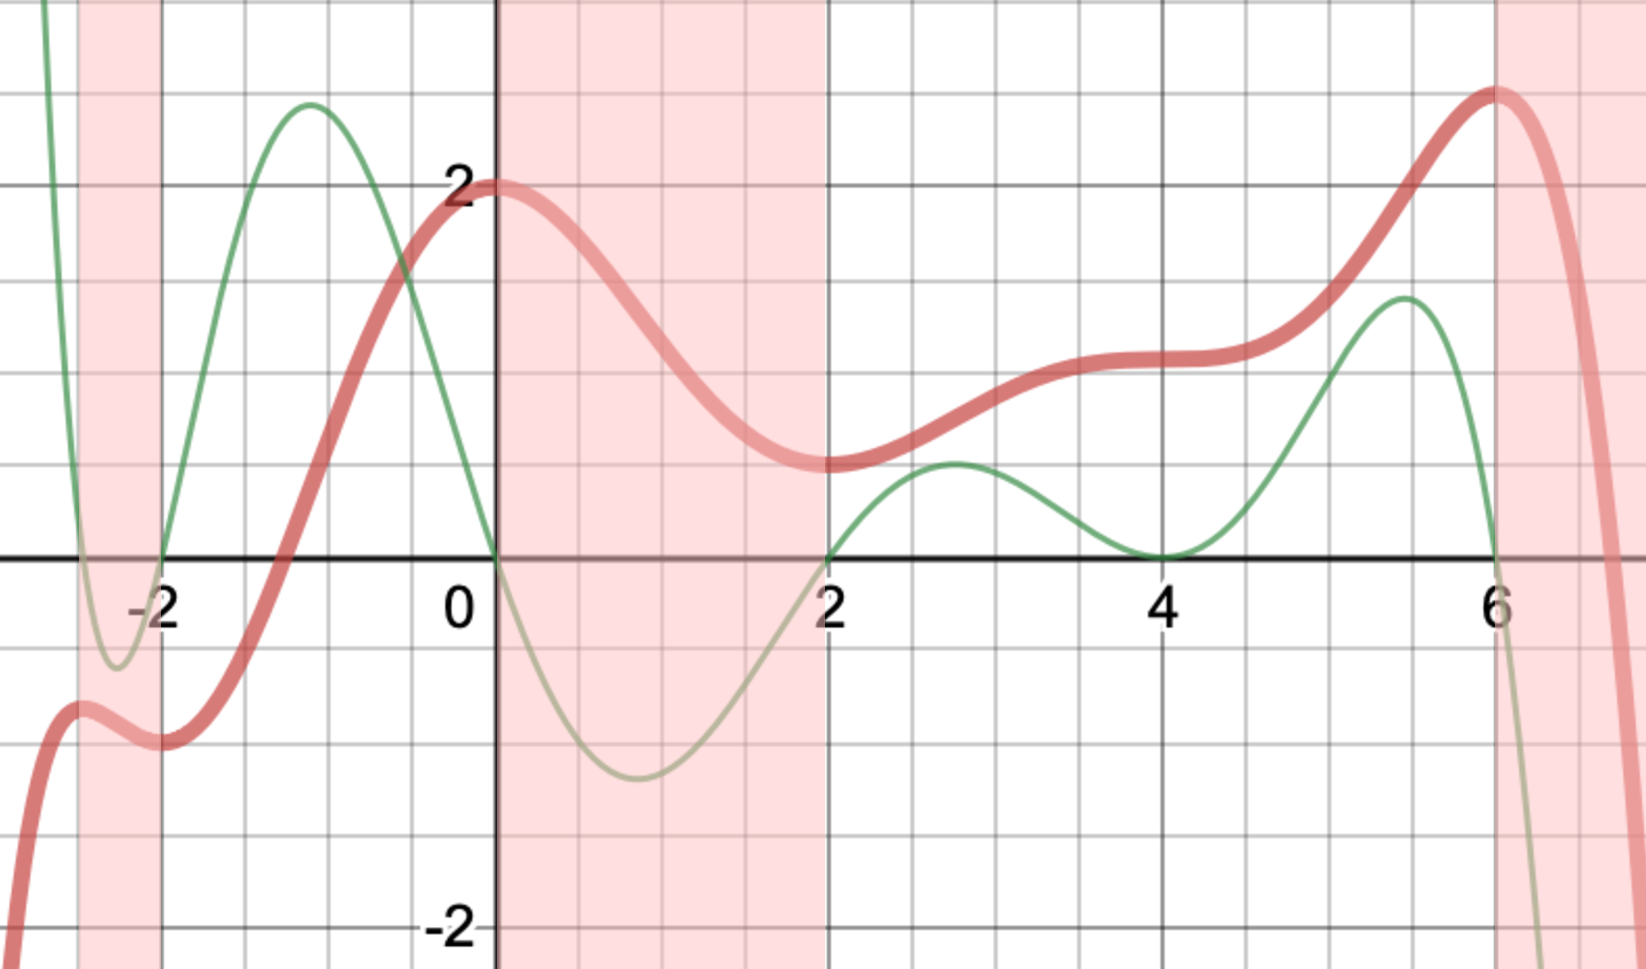
\includegraphics[width=8cm]{pic/Kurdi2.pdf}
\end{center}
\caption{Intervals where the function is decreasing}
\label{figkurvdiss2}
\end{figure}

Note that at the points where increasing/decreasing changes (that is where
the derivative is zero), the function has a local maximum or minimum.
``Local'' here
means that it is larger than at any other point in the neighborhood, though
it might be even larger somewhere away\mynote{In the same way as the tallest
person in town is not guaranteed to be the tallest person in the country}.
\begin{defn}
A point $x_0$, where $f'(x_0)=0$ is called a \defini{critical point} for
$f$.
\end{defn}
We have seen that (local) maxima and minima occur only at critical points,
namely a maximum if the derivative changes from positive to negative, and a
minimum if the derivative changes from negative to positive.

In the example we have critical points at $-2.5$,$0$,and $6$ (maxima) as
well as at $-2$ and $2$ (minima).

But there is a further critical point,
namely we have $f'(4)=0$. Here the derivative becomes zero, but does not
change its sign (i.e. stays nonnegative). What happens is that the function
briefly stops growing\mynote{like a mountain climber who briefly stops to
catch a deep breath} but then immediately grows again. Such a point is
called a \defini{saddle point}.

We can distinguish easily between the three kinds of critical points, if we
also look at the second derivative. At a maximum, the derivative was
positive and becomes negative, so the second derivative must be negative.
At a minimum, with an analogous argument, the second derivative is positive.
And at a saddle point, the derivative becomes zero but does not change its
sign. That means a saddle point is a local minimum or maximum of the
derivative, and thus must have the second derivative zero as well.
\subsection{Turning Points}

Let us now look at the general impact of the second derivative.
Figure~\ref{figkurvdiss3} now shows first (green) and second (blue)
derivative, as well as an indication of the places where the derivatives
become zero.
\begin{defn}
A point $x_0$, where the second derivative is zero,
$f^{\prime\prime}(x_0)=0$ is called a \defini{turning point} (or
\defini{inflection point}) for $f$.
\end{defn}

\begin{figure}
\begin{center}
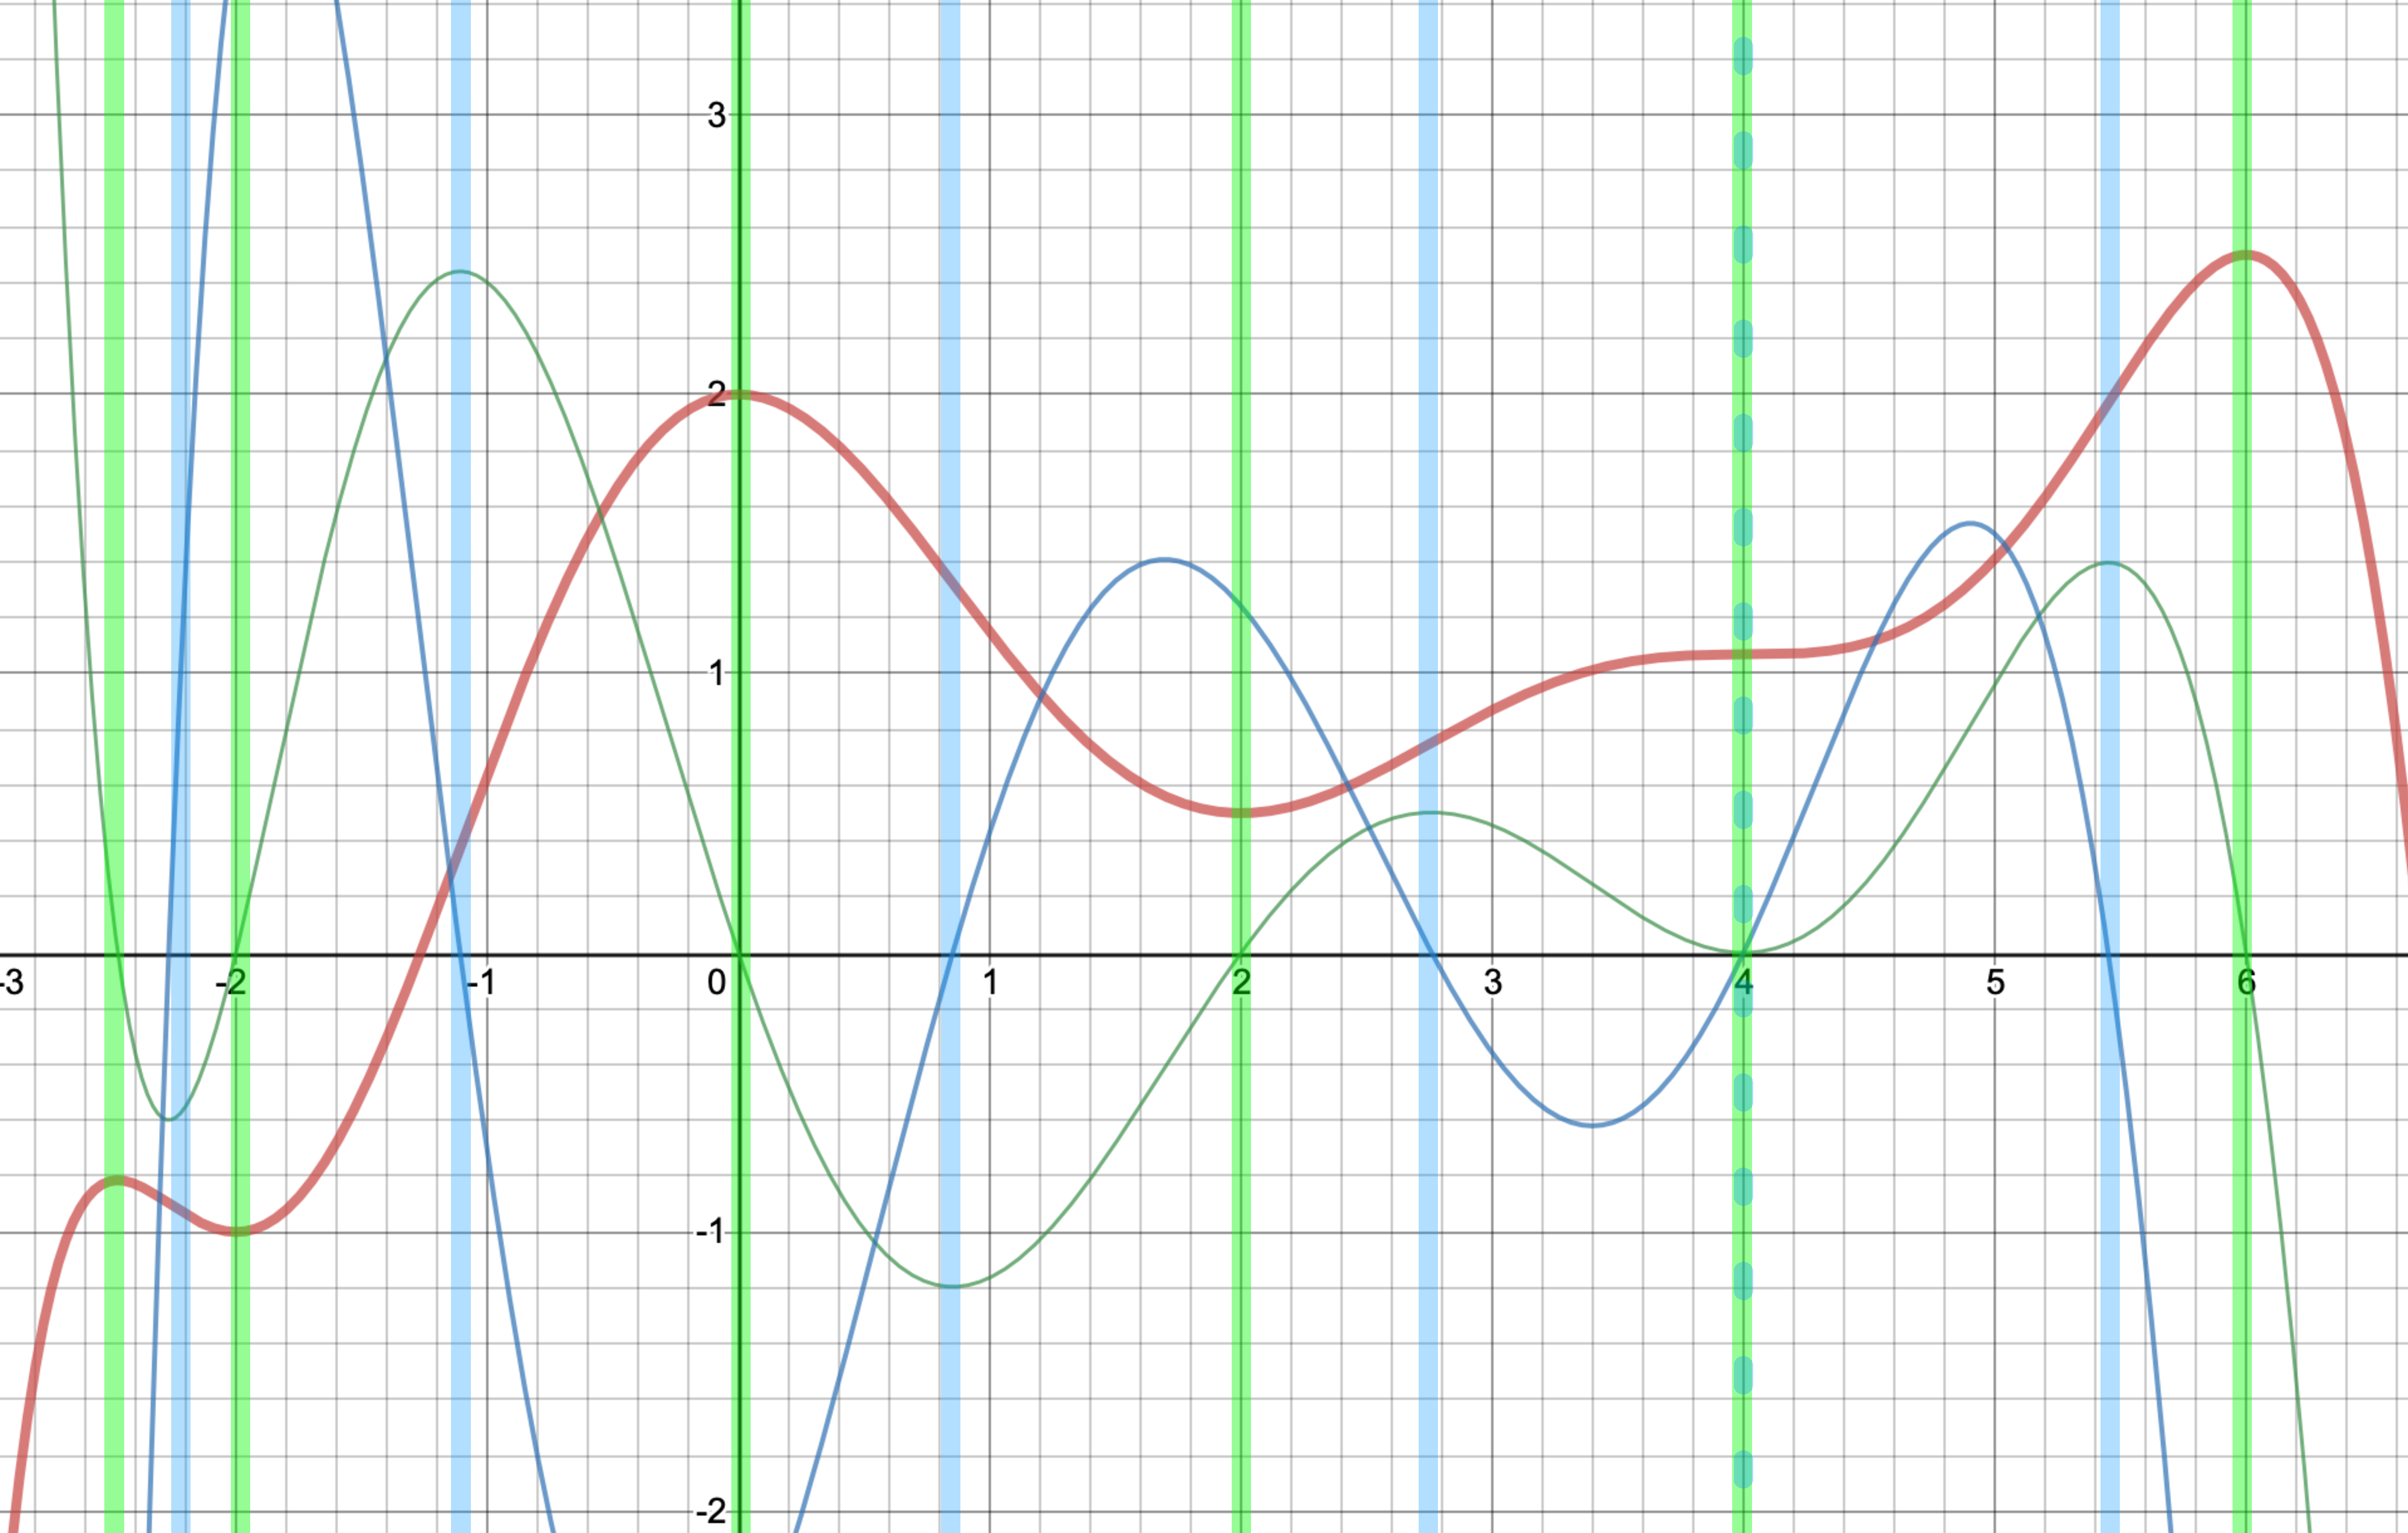
\includegraphics[width=8cm]{pic/Kurvendiskussion.pdf}
\end{center}
\caption{Critical and Turning points}
\label{figkurvdiss3}
\end{figure}
We see that when the second derivative is positive, the derivative becomes
larger and the growth of the function increases. The graph of the function
is therefore \defini{convex}, that is it turns left.
(Some textbooks use ``concave down'' in place of ``convex''.) Similarly, the
graph is \defini{concave}, that is it turns right, if the second derivative
is negative. 
At turning points, when the second derivative changes its sign, the graph of
the function changes from left turn to right turn, or vice versa.
\medskip

Let us summarize these observations on the shape of $f$ in
table~\ref{tabkurdi}. The middle column describes critical points, the
second and fourth row turning points.
\begin{table}
{\hyphenpenalty=10000
\begin{center}
\begin{tabular}{p{17mm}|p{25mm}|p{25mm}|p{25mm}}
&$f'(x_0)>0$&
$f'(x_0)=0$, {\em Critical Point}&
$f'(x_0)<0$\\
\hline
$f^{\prime\prime}(x_0)<0$&
\begin{raggedright}
$f$ increases and is convex.
\centerline{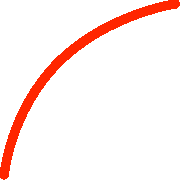
\includegraphics[width=16mm]{pic/CTL.pdf}}
\end{raggedright}&%
\begin{raggedright}
$f$ reaches a maximum.
\centerline{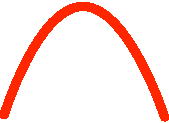
\includegraphics[width=16mm]{pic/CMA.pdf}}
\end{raggedright}&%
\begin{raggedright}
$f$ decreases and is convex.
\centerline{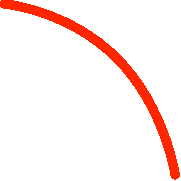
\includegraphics[width=16mm]{pic/CTR.pdf}}
\end{raggedright}
\\

\hline
\begin{raggedright}%
$f^{\prime\prime}(x_0)=0$
{\footnotesize 
and $f^{\prime\prime}$ changes from $-$ to $+$. (I.e.
$f^{\prime\prime\prime}(x)>0$)}
{\em Turning Point}
\end{raggedright}&
\begin{raggedright}
$f$ increases and has a turning point
from right to left
\centerline{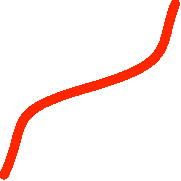
\includegraphics[width=16mm]{pic/CUL.pdf}}
\end{raggedright}&%
\begin{raggedright}
$f$ has a saddle point, increasing.
$f'$ stays positive
\centerline{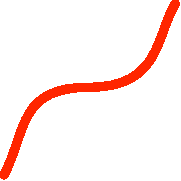
\includegraphics[width=16mm]{pic/CSU.pdf}}
\end{raggedright}&%
\begin{raggedright}
$f$ decreases and has a turning point
from right to left
\centerline{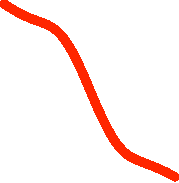
\includegraphics[width=16mm]{pic/CDL.pdf}}
\end{raggedright}\\

\hline
$f^{\prime\prime}(x_0)=0$ constant zero&
\begin{raggedright}
$f$ increases straight. $f'$ is constant.
\centerline{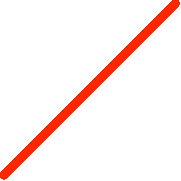
\includegraphics[width=16mm]{pic/CIN.pdf}}
\end{raggedright}&%
\begin{raggedright}
$f$ is constant.
\centerline{
\includegraphics[width=16mm]{pic/CCO.pdf}}
\end{raggedright}&%
\begin{raggedright}
$f$ decreases straight. $f'$ is constant.
\centerline{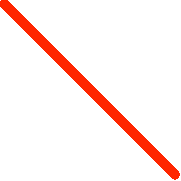
\includegraphics[width=16mm]{pic/CDE.pdf}}
\end{raggedright}
\\

\hline
\begin{raggedright}%
$f^{\prime\prime}(x_0)=0$
{\footnotesize 
and $f^{\prime\prime}$ changes from $+$ to $-$. (I.e.
$f^{\prime\prime\prime}(x)<0$)}
{\em Turning Point}
\end{raggedright}&
\begin{raggedright}
$f$ increases and has a turning point
from left to right
\centerline{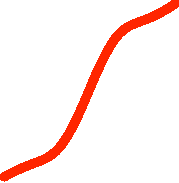
\includegraphics[width=16mm]{pic/CUR.pdf}}
\end{raggedright}&%
\begin{raggedright}
$f$ has a saddle point, decreasing.
$f'$ stays negative
\centerline{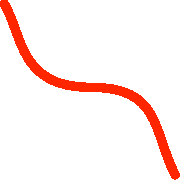
\includegraphics[width=16mm]{pic/CSD.pdf}}
\end{raggedright}&%
\begin{raggedright}
$f$ decreases and has a turning point
from left to right
\centerline{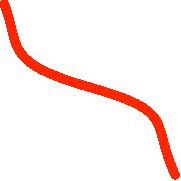
\includegraphics[width=16mm]{pic/CDR.pdf}}
\end{raggedright}\\

\hline
$f^{\prime\prime}(x_0)>0$&
\begin{raggedright}
$f$ increases and is concave.
\centerline{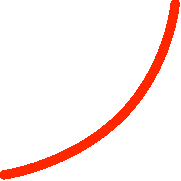
\includegraphics[width=16mm]{pic/CBR.pdf}}
\end{raggedright}&%
\begin{raggedright}
$f$ reaches a minimum.
\centerline{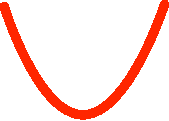
\includegraphics[width=16mm]{pic/CMI.pdf}}
\end{raggedright}&%
\begin{raggedright}
$f$ decreases and is concave.
\centerline{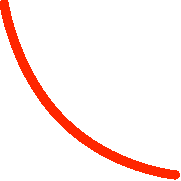
\includegraphics[width=16mm]{pic/CBL.pdf}}
\end{raggedright}
\\

\end{tabular}
\end{center}
}
\caption{The local shapes of a curve}
\label{tabkurdi}
\end{table}

Using this table, we now can describe the shape of the graph of a function,
though it does not allow us to determine absolute function values or
decide on tie-breaks amongst local maximal/minima which ones are larger.

Note that there is a symmetry between a function and its negative (flipped
upside down), and both will have the same critical points and turning
points. We thus need to have at least one information about a
derivative value being positive or negative to be able to distinguish
between these two cases.
\smallskip

Let us do this for the function in the example. Using the zeroes of the two
derivatives (the colored vertical lines in Figure~\ref{figkurvdiss3}), we
split the domain from $-3$ to $7$ into intervals. We indicate the type as
\textbf{C}ritical or \textbf{T}urning. Note how two critical points are
separated by turning points.
\[
\begin{array}{lc|c|c}
x&\mbox{Type}&f('(x)&f^{\prime\prime}(x)\\
\hline
&&+&-\\
-2.5&C&0&-\\
&&-&-\\
-2.2&T&-&0\\
&&-&+\\
-2&C&0&+\\
&&+&+\\
-1.1&T&+&0\\
&&+&-\\
0&C&0&-\\
&&-&-\\
0.85&T&-&0\\
\end{array}\qquad
\begin{array}{lc|c|c}
x&\mbox{Type}&f('(x)&f^{\prime\prime}(x)\\
\hline
&&-&+\\
2&C&0&+\\
&&+&+\\
2.75&T&+&0\\
&&+&-\\
4&CT&0&0\\
&&+&+\\
5.45&T&+&0\\
&&+&-\\
6&C&0&-\\
&&-&-\\
\\
\end{array}
\]
We now can (Figure~\ref{figfuncsynth}) find the corresponding local shapes in the table and compose them
to approximate the overall shape of the function graph.
\begin{figure}
\begin{center}
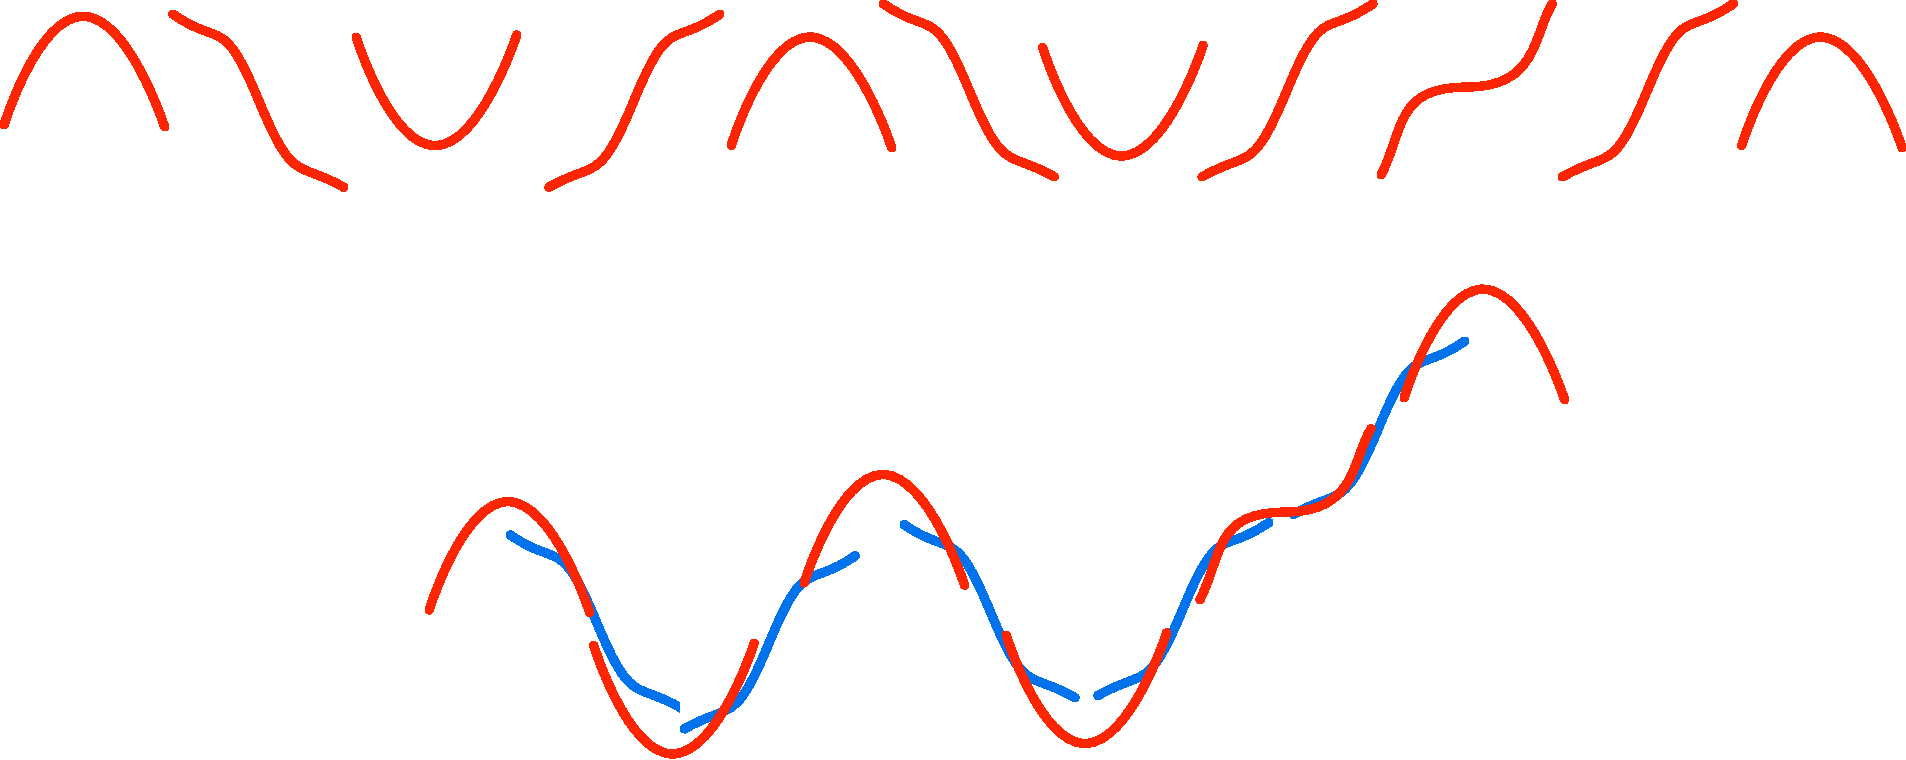
\includegraphics[width=8cm]{pic/FuncSynth.pdf}
\end{center}
\caption{Composing local shapes}
\label{figfuncsynth}
\end{figure}

\bigskip


The advantages of using the derivative over other potential methods are:
\begin{itemize}
\item No plot is needed.
\item One can find the relevant points exactly
\item Identifying a point where a derivative is zero is often easier than
identifying the point of a maximum or minimum\mynote{Imagine a pool in which
the water level is changing. It is easier to see when the water level is
crossing a threshold than when it is maximal.}
\item One can solve the problem, even if the definition of the function
involves other variable parameters (and one thus cannot plot).
\end{itemize}

\begin{bsp}
%TN, edited AH

For a more complicated example, consider the function $f(x) = x^2e^{-x}$.
Let's find the critical points, turning points, and determine where the function is increasing/decreasing and where it is concave up/down. 

First we find the critical points. To do that we need to find the derivative $f'(x)$:
\begin{equation*}
\begin{split}
f'(x) &= \big(x^2e^{-x}\big)' \\
&= (x^2)'e^{-x} + x^2(e^{-x})' \quad \text{(product rule)} \\
&= 2xe^{-x}x^2 + x^2(-e^{-x}) \quad \text{(power rule on }x^2 \text{, chain rule on }(e^{-x})' \text{)} \\
&= (2x-x^2)e^{-x} \quad \text{(simplification)}.
\end{split}
\end{equation*} 
Now we solve $f'(x) = (2x-x^2)e^{-x} = 0$. The factor $e^{-x}$ is never zero
so we just need to find the zeros of $2x-x^2$, which are $x=0$ and $x=2$.
These are the (only!) critical points.

Now we figure out where $f(x)$ is increasing and decreasing. This is
determined by the sign of $f'(x)$, which must stay the same outside the
critical points. We thus consider $f'(x)$  on the intervals $(-\infty,0), (0,2), (2,\infty)$.
From
a calculator we find $f'(-1) \approx -8.15$, so $f'$ is negative at $x=-1$,
and thus $f$ is decreasing for $x<0$.
Similarly, we calculate $f'(1) \approx 0.3679$ and thus have $f$ increasing
for $0<x<2$. And
$f'(3) \approx -0.1494$ so $f(x)$
must be decreasing again for $2<x$. This together tells us that $f$ has a
local minimum at $x=0$ and a
local maximum at $x=2$.

Now we find turning points and think about concavity. Toward that end we will
need $f''(x)$: \begin{equation*} \begin{split} f''(x) &= ((2x-x^2)e^{-x})' \\
&= (2x-x^2)'e^{-x} + (2x-x^2)(e^{-x})' \quad \text{(product rule)} \\ &=
(2-2x)e^{-x} + (2x-x^2)(-e^{-x}) \quad \text{(power rule and chain rule)}\\
&= (x^2-4x+2)e^{-x} \quad \text{(simplification)}.  \end{split}
\end{equation*}
Again the factor $e^{-x}$ is never zewro and we thus only need to consider
the polynomial $x^2-4x+2$. Its roots are
$x=2-\sqrt{2} \approx 0.586$ or $x=2+\sqrt{2} \approx 3.414$. These
are the turning points. A calculator gives us  that
$f''(0) = 2$, $f''(2) \approx -.2707, f''(4) \approx 0.0366$, thus
$f(x)$ is concave up for $x<2-\sqrt{2}$, concave down for
$(2-\sqrt{2}<x<2+\sqrt{2})$ and concave up for $2+\sqrt{2}<x$.
A look at the graph of $f(x)$ in Figure~\ref{tnex3fig} illustrates this.
\begin{figure}
\begin{center}
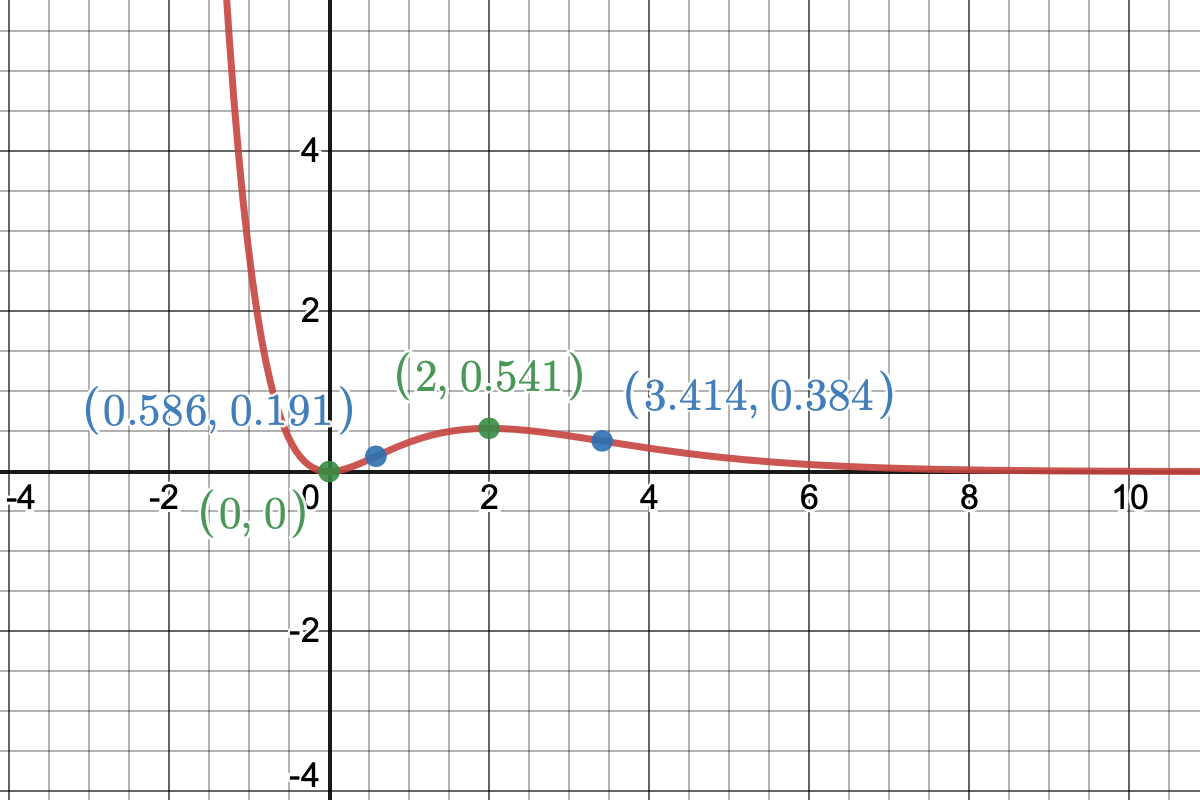
\includegraphics[width=8cm]{pic/tnex3pic.png}
\end{center}
\caption{The graph of $x^2\cdot e^{-x}$ with critical points and turning
points.}
\label{tnex3fig}
\end{figure}
\end{bsp}


\section{Optimization}

An important application for finding maxima/minima is in optimization. We
are considering a problem that involves a parameter that can be chosen, and
have a cost function whose value we want to minimize (or a ``gain'' function
we want to maximize), that means we look for the maximum or minimum of a
function.
\smallskip

As we have seen, these extrema must happen at critical points. We just need
to decide which ones are maxima, which ones minima, and, if there are
several, which ones are best. Furthermore, if the set of valid parameter
values if not the whole real axis, it is possible that a maximum/minimum is
reached at the maximal/minimal parameter values: The function $f(x)=x+1$ has,
for values $2\le x\le 5$ the maximal value $6$ at $x=5$, though this is not
even a critical point.
\medskip

Let us consider this in an example:

We have a fence of 100 units length and want to use it to surround a
rectangular area that is as large as possible. Assuming we use the whole
fence, we denote the length of one side (and the opposite side) by $x$, then
the other two sides\mynote{It is $50-x$ and not
$100-x$ as there are two sides in each direction.}
both have length $50-x$.

The area of the rectangle then is $f(x)=x\cdot(50-x)=50x-x^2$ square units,
and the permitted values for $x$ are from $0$ to $50$ (in both end cases the
rectangle degenerates to a line).
\smallskip

To find the critical points, we calculate $f'(x)=50-2x$ and find $x=25$ is
the only critical point. Since $f(25)=25^2=625>0$ and $f(0)=0=f(50)$ this is
a maximum and the global maximum. The best fence thus has one side of length
25 (and thus the other side also of length $50-25=25$).
\medskip

For a more involved problem, imagine that the manufacturer {\em Consolidated
Widgets} decides to produce a new exquisite widget, using their trademark
{\em magic dust}. Due to the interaction of the magic dust with the other
ingredients, the manufacturing cost of a widget containing $x$ units of dust
is $f(x)=x^3-50x^2+700x-1000$ doubloons. To be exquisite, the widget also needs
to contain at least $5$ units of dust, and can contain at most $50$ units.
For which amount of dust is the
manufacturing cost per widget minimal?

Again, we consider the derivative $f'(x)=3x^2-100x+700=(x-10)(3x-70)$. The
critical points thus are $10$ and $70/3\sim 23.33$. We now evaluate $f(x)$
at the critical points, as well as the end points:
\[
\begin{array}{c|r|r|r|r}
x&5&10&23.33&50\\
\hline
f(x)&1375&2000&814.81&34000\\
\end{array}
\]
We find that the minimal manufacturing cost (namely $814.81$) is obtained when using $23.33$
units of dust per widget (while the maximum cost would be for $50$ units).

\section{Newton's Method}
\label{secnewton}

We go back to the problem already studied in Section~\ref{secwhycont} on how
to find (an approximation of) $x_0$ such that $f(x_0)=0$.
We had seen that the method of halving intervals required $\log_2(10)\sim
3.3219$ steps in average for each extra digit of accuracy in the
approximation -- in the example we got an error $<10^{-6}$ (i.e. $6$ decimal
digits) after 20 iterations.
This is far too bad for many practical applications, and we want to try
better. 

The problem of the interval halving method is that it always goes to the
middle of the interval, while the actual point $x_0$ with $f(x_0)=0$ might
be far closer to the a side of the interval. Figure~\ref{fignewton4}, for
example, shows four different functions on the interval $[2,5]$, all of
which have $f(2)=1$ and $f(5)=-1$ (and thus a zero in the interval), but the
placement of the zeroes is quite different. The left or right side of the
interval thus might not be a much better approximation of the root.
\begin{figure}
\begin{center}
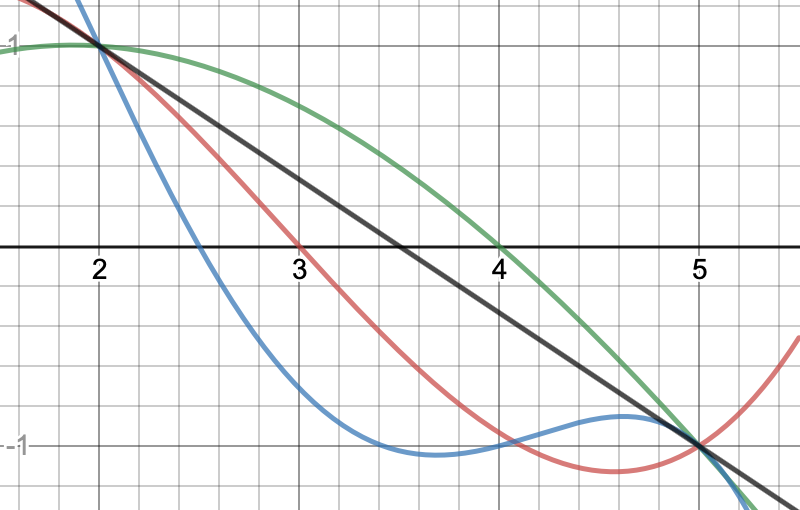
\includegraphics[width=8cm]{pic/newton4.png}
\end{center}
\caption{Different placement of zeroes}
\label{fignewton4}
\end{figure}

The idea of the Newton method is to not just consider halved intervals
as a good approximation, but use the tangent line (whose slope
indicates how steep the function is) to find a better
approximation\mynote{That is, to find a valley, we go downhill}. That
is, if we have a point $x_n$ as approximation of the root, we follow the
tangent to $f$ at $x_n$ (whose slope is $f'(x_n)$) to the point where it
intersects the $x$-axis, and take that $x$-value as the next approximation
$x_{n+1}$. Figure~\ref{fignewtonm} illustrates this process.

\begin{figure}
\begin{center}
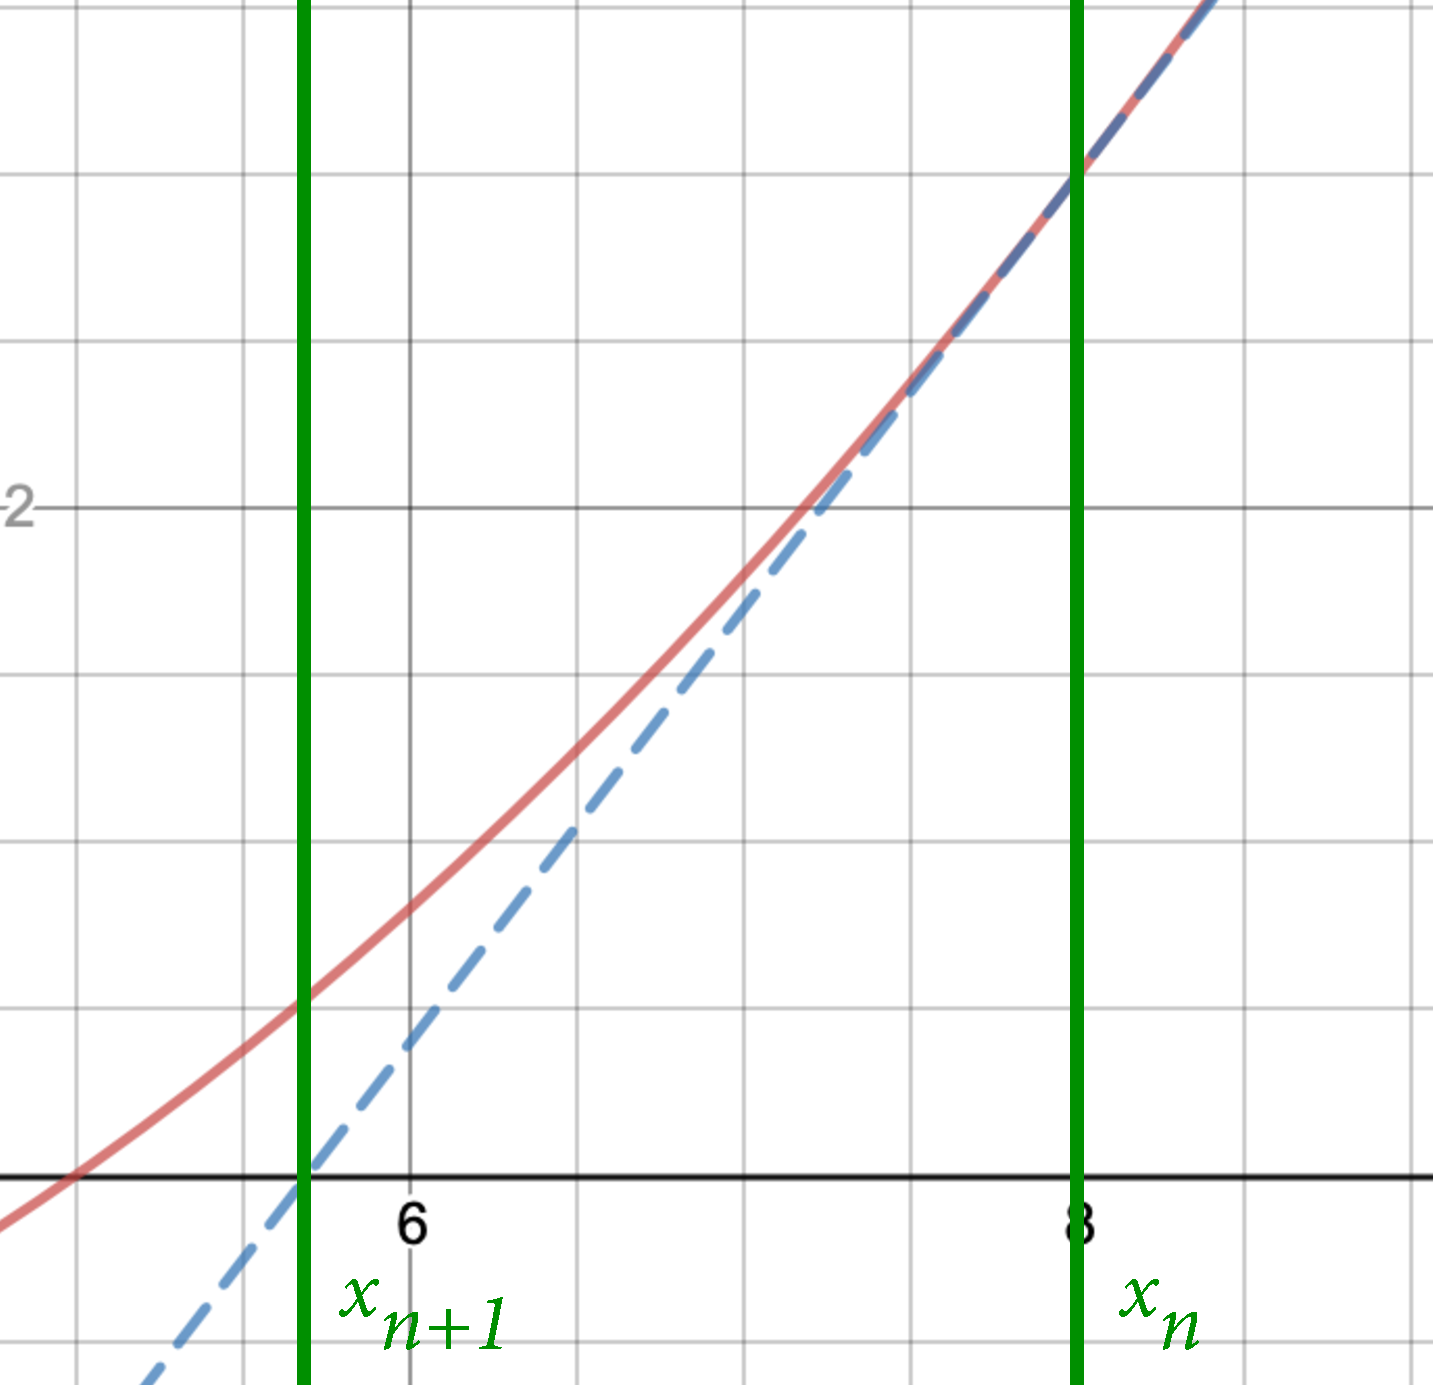
\includegraphics[width=6cm]{pic/newtonmeth.pdf}
\end{center}
\caption{The Newton Method}
\label{fignewtonm}
\end{figure}

To find a formula for $x_{n+1}$ observe that the tangent line goes through
the points $(x_{n+1},0)$ and $(x_n,f(x_n))$ and has slope $f'(x_n)$. Thus
\[
f'(x_n)=\frac{f(x_n)-0}{x_n-x_{n+1}}
\]
and we solve (assuming that $f'(x_0)\not=0$) for
\[
x_{n+1}=x_n-\frac{f(x_n)}{f'(x_n)}
\]
Let us look at this in the same example as we did for the halving method. We
take $f(x)=\sin(x)$ and start at $x_0=2$. The formula gives us the recursion
\[
x_{n+1}=x_n-\frac{\sin(x_n)}{\cos(x_n)}
\]
and we calculate values as
\begin{eqnarray*}
&x_0=2, \quad x_1=4.185039863,\quad x_2=2.467893675, \quad x_3=3.266186277&\\
&x_4=3.140943912, \quad x_5=3.141592654,\quad x_6=3.141592654&\\
\end{eqnarray*}
Note that after 5 iterations (instead of 20 before) we approximated the zero
to $6$ digits. Even more, at that point we actually have it approximated
already to 9 digits!

This is not just happenstance. One can show that, as long as the starting
value is not too far away for the root, the Newton method converges
quadratically, that (up to a constant) the error after each step is bounded
by the square of the previous error. That means that the number of correct
digits after each step will increase by a factor (in the above example it
seems to be roughly 2), while for the interval halving method it only
increased by one digit every three steps. This shows that the Newton
method is far more powerful than interval halving.

\section{Indefinite Limits and L'Hospital's rule}

For reasons we shall see in the next section, we want to be able to
calculate limits of quotients.

We have see the limit rule for quotients that (in a version for
functions) gives us that for a number $a$ (or $a=\infty$) and functions
$f,g\colon\R\to\R$ we have
\[
\lim_{x\to a}\frac{f(x)}{g(x)}=\frac{\lim_{x\to a}f(x)}{\lim_{x\to a}g(x)},
\]
if the fraction of limits on the right hand side exists. But what if
numerator and denominator on the right hand side are both $0$? Or both
$\infty$? An answer to this question is given by a test that is
called\mynote{Not after the inventor, but after a popularizer of it}
L'Hospital's rule (pronounced {\em lowpytaal's} rule).

\begin{thm}
Let $f,g\colon\R\to\R$ be differentiable functions and $a\in\R$ or
$a=\infty$ such that $\lim_{x\to a}f(x)=0\lim_{x\to a}g(x)$, respectively
$\lim_{x\to a}f(x)=\infty\lim_{x\to a}g(x)$. Then, if $\lim_{x\to
a}\frac{f'(x)}{g'(x)}$ exists, we have that
\[
\lim_{x\to a}\frac{f(x)}{g(x)}=\lim_{x\to a}\frac{f'(x)}{g'(x)}.
\]
\end{thm}
The reader surely will have noted that this quotient of derivatives is {\em
not} the derivative of the quotient!\\
\begin{proof}
We give a proof only for the case that $a\in\R$ and $f(a)=0=g(a)$ and that
$f'(x)$ and $g'(x)$ are continuous at $a$. (The other cases are
significantly harder.) Then
\begin{eqnarray*}
\lim_{x\to a}\frac{f(x)}{g(x)}
&=&\lim_{x\to a}\frac{f(x)-0}{g(x)-0}
=\lim_{x\to a}\frac{f(x)-f(a)}{g(x)-g(a)}\\
&=&\lim_{x\to a}\frac{\frac{f(x)-f(a)}{x-a}}{\frac{g(x)-g(a)}{x-a}}
=
\frac{\lim_{x\to a}\frac{f(x)-f(a)}{x-a}}{\lim_{x\to
a}\frac{g(x)-g(a)}{x-a}}\\
&=&\frac{f'(a)}{g'(a)}=\lim_{x\to a}\frac{f'(x)}{g'(x)}.
\end{eqnarray*}
\end{proof}

For example, we have that
\[
\lim_{x\to\infty}\frac{x-1}{x^2-1}=
\lim_{x\to\infty}\frac{1}{2x}=0
\]

Note that a situation of $\infty/\infty$ can give us finite (nonzero)
limits. For example
\[
\lim_{x\to\infty}\frac{3x-5}{73-15}=
\lim_{x\to\infty}\frac{3}{7}=\frac{3}{7}
\]

It is possible to apply L'Hospital's rule multiple times. In the following
example, the first application of L'Hospital's rule still leaves us with an
$\infty/\infty$ case, but the second one then gives the value:
\[
\lim_{x\to\infty}\frac{4x^2+3x-1}{5x^2-x+1}
=\lim_{x\to\infty}\frac{8x+3}{10x^2-1}
=\lim_{x\to\infty}\frac{8}{10}=\frac{4}{5}.
\]
More generally, if we have a quotient of polynomials, we need to apply 
L'Hospital's rule as many times as (the smaller of) the degrees of numerator
and denominator:
\begin{thm}
Let $f(x),g(x)$ be nonzero polynomials. Then limit of the quotient
\[
\lim_{x\to\infty}\frac{f(x)}{g(x)}
\]
equals:
\begin{description}
\item[$0$] if the degree of $g(x)$ is larger than the degree of $f(x)$.\\
\item[$\pm\infty$] if the degree of $f(x)$ is larger than the degree of
$g(x)$\\
\item[$a/b$] if the degree of $f$ equals the degree of $g$, and $a$ is the
leading coefficient of $f$ and $b$ the leading coefficient of $g$.
\end{description}
\end{thm}
The same statement obviously also holds with $n$ in place of $x$ and
explains the limits of sequences we observed earlier.

\begin{bsp}
%TN edited AH
Note that even if L'Hospitals rule is applicable, there is no guarantee that
the result is helpful for solving the problem.
Consider the limit
\[\lim_{x \to \infty}\frac{e^x-e^{-x}}{e^x+e^{-x}}.\]
It is easy to see that $e^x-e^{-x} \to \infty$ and $e^x+e^{-x} \to \infty$ as
$x \to \infty$, so it is valid to apply L'Hospital's rule here. But if we do,
we find
\[
\lim_{x \to \infty}\frac{e^x-e^{-x}}{e^x+e^{-x}} = \lim_{x \to
\infty}\frac{\frac{d}{dx}(e^x-e^{-x})}{\frac{d}{dx}(e^x+e^{-x})} = \lim_{x
\to \infty}\frac{e^x+e^{-x}}{e^x-e^{-x}}.
\]
This limit really doesn't seem
any simpler. Indeed, if we try L'Hospital's rule again we find
\[
\lim_{x \to
\infty}\frac{e^x+e^{-x}}{e^x-e^{-x}} = \lim_{x \to
\infty}\frac{\frac{d}{dx}(e^x+e^{-x})}{\frac{d}{dx}(e^x-e^{-x})} = \lim_{x
\to \infty}\frac{e^x-e^{-x}}{e^x+e^{-x}}
\]
which is where we started! We can
keep trying to apply L'Hospital's rule, but we'll simply alternate back and
forth between these equally-difficult-to-compute limits. 
\end{bsp}

\section{Order of growth}

\def\bigo#1{{\cal O}\/\left(#1\right)}
\begin{defn}
For two functions $f,g\colon\R\to\R$, we say that $f$ is of \defini{order
of} $g$ (or $f$ is \defini{big O} of $g$) if there exists $c,N\in\R$, such
that $\sz{f(x)}\le c \sz{g(x)}$ for all $x\ge N$. We write
$f(x)=\bigo{g(x)}$.
\end{defn}

If $f(x)=\bigo{g(x)}$, this means that behavior of $f$ for large values of
$g$ is dominated by the behavior of $g$.

For example, we have that $x^2+5x=\bigo{x^2}$, since for $x\ge 5$ we have
that $x^2\ge 5x$ and thus $\sz{x^2+5x}\le x^2+x^2=2x^2$.
\medskip

This notation is often used when
comparing the performance of algorithms. Here $f(n)$
\mynote{It is
common to give these classes as functions of a variable $n$, rather than
$x$}
is a
function that, for a given algorithm indicates the cost (number or
operations) required for an input that has size $n$. If there is a second
algorithm, whose cost is given by a function $g$, we consider the first
algorithm as not worse than the second, if $f(x)=\bigo{g(x)}$. If in
addition $g(x)=\bigo{f(x)}$, the algorithms are considered
equivalent.\mynote{There is a plethora of variants of $\bigo{}$ that provide
modified kinds of comparisons.}
\smallskip

The justification for such reasoning is that the constant $c$ will make such
a comparison independent of particular computers or programming
languages used. The focus on large values of the input size allows us to
ignore artifacts for small examples, or effects such as caching or results.
The use of the $\bigo{}$ notation also allows us to focus an the main
contribution to an algorithms runtime.

For example, when searching an object in a list of length $l$, a linear
search has cost $\bigo{n}$ (go through the list until you find the object),
while if the list is sorted a binary search has only cost $\bigo{\log(n)}$,
which we shall see is much better.
%sorting a list of $n$ objects, bubble sort (a double for
%loop comparing adjacent pairs) has run time $\bigo{n^2}$, while quick sort
\medskip

The test for $f(x)=\bigo{g(x)}$ looks a little bit like the criterion for
limit of a series, and proving it might be technical. The following theorem
shows that this can be tested easier in many cases:
\begin{thm}
\label{thmgo}
Let $f,g\colon\R\to\R$ be two functions such that 
$L=\displaystyle \lim_{x\to\infty}\frac{f(x)}{g(x)}$ exists. Then
\begin{itemize}
\item[a)] if $L=0$ then $f(x)=\bigo{g(x)}$
\item[b)] if $L=\infty$ then $g(x)=\bigo{f(x)}$.
\item[c)] if $0<L\not=\infty$ is a finite number then 
$f(x)=\bigo{g(x)}$ \textbf{and} $g(x)=\bigo{f(x)}$.
\end{itemize}
\end{thm}
The proof of a) is basically to apply the definition of a limit, and to multiply
by the denominator $g(x)$, this will yield the criterion for $\bigo{}$. For
b) and c) also consider the reciprocal fraction $g(x)/f(x)$.
\begin{note}
The criteria in this theorem are sufficient, but not necessary. For example
consider $f(x)=\sin(x)$ and $g(x)=1\cdot x^0$. Then clearly
$\sin(x)=\bigo{1}$ (choose constants $c=1$ and $N=1$), but the limit
$\displaystyle \lim_{x\to\infty}\frac{\sin(x)}{1}$ does not exist.
\end{note}

An important consequence of this theorem is the following observation, that
allows to ignore ``lower order'' terms as ``noise'':

Suppose that $f(x)=\bigo{g(x)}$ and $h(x)=\bigo{f(x)}$. Then\mynote{Since,
by the limit rules,
$\displaystyle \frac{f(x)+h(x)}{g(x)}=\frac{f(x)}{g(x)}\left(1+\frac{h(x)}{f(x)}\right)$
and $\displaystyle\lim_{x\to\infty}\left(1+\frac{h(x)}{f(x)}\right)=1$.}
$f(x)+h(x)=\bigo{g(x)}$.

Thus, for example, setting $f(x)=g(x)=x^3$, $h(x)=9x^2+17+\log(x)$,
we get that $x^3+9x^2+17+\log(x)=\bigo{x^3}$.

\subsection{Complexity classes}
The criterion of Theorem~\ref{thmgo} is often ready-made for using
L'Hospital's theorem. For example let $f(x)=x+1$ and $g(x)=x^2-3x+2$.
We have that
\[
\lim_{x\to\infty}\frac{x+1}{x^2-3x+2}
=\lim_{x\to\infty}\frac{1}{2x-3}=0
\]
Thus $x+1=\bigo{x^2-3x+2}$.

The same argument will work for {\em any} pair of polynomials of degree 1
and 2.
\smallskip

Indeed, by applying L'Hospital's theorem several times, we find that if
$f(x)$ is a polynomial of degree $m$, and $g(x)$ a polynomial of degree
$n\ge m$ then $f(x)=\bigo{g(x)}$. In particular (setting $g(x)=x^m$) we have
that $f(x)=\bigo{x^m}$.

More generally, we get that for $a,b>0$ with $a<b$ that $x^a=\bigo{x^b}$ but
{\em not} vice versa.
\smallskip

We similarly compare a power $x^a$ (for $a>0$) to $\exp(x)$ and to $\log(x)$
(we give the argument for $a\in\Z$, the argument for non-integral $a$ is very
similar):
\begin{eqnarray*}
\lim_{x\to\infty}\frac{x^a}{\exp(x)}&=&
\lim_{x\to\infty} \frac{a\cdot x^{a-1}}{\exp(x)}=\cdots=
\lim_{x\to\infty} \frac{a\cdot(a-1)\cdots 1\cdot x^{a-a}}{\exp(x)}\\
&=&
\lim_{x\to\infty} \frac{a!}{\exp(x)}=0,
\end{eqnarray*}
so $x^a=\bigo{\exp(x)}$. Similarly
\begin{eqnarray*}
\lim_{x\to\infty}\frac{\log(x)}{x^a}&=&
\lim_{x\to\infty}\frac{1/x}{a\cdot x^{a-1}}=
\lim_{x\to\infty}\frac{7}{a\cdot x^a}=0
\end{eqnarray*}
and thus $\log(x)=\bigo{x^a}$.

We thus get a hierarchy of function classes that all have different growth
(and thus would describe different algorithmic performance).
We summarize this in Table~\ref{tabcomplcla} and Figure~\ref{figcomcl}.
\begin{table}
\begin{tabular}{p{24mm}|p{30mm}|p{40mm}}
&Name&Example algorithm in class\\
\hline
$\bigo{1}$&constant, or bounded&Append to a list\\
$\bigo{\log(n)}$&logarithmic&Binary search in sorted list\\
$\bigo{n^c}$, $0<c<1$&sublinear, or fractional power&Testing $n$ for primality by trial division\\
$\bigo{n}$&linear&Searching through an unsorted list\\
$\bigo{n\log(n)}$&superlinear&Merge sort\\
$\bigo{n^c}$, $1<c<2$&&\\
$\bigo{n^2}$&quadratic&Bubble sort\\
$\bigo{n^c}$, $2<c<3$&&\\
$\bigo{n^3}$&cubic&Solving a system of $n$ linear equations (standard
method)\\
$\bigo{n^c}$, $3<c$&&\\
&{\em All up to here are called ``polynomial time''}&\\
$\bigo{\exp(n^c)}$, $0<c<1$&subexponential&Best known factorization of
$n$-digit number.\\
$\bigo{\exp(n)}$&exponential&Brute-force breaking of a password of length $n$\\
$\bigo{n!}$&factorial&Traveling salesman by trying out all tours\\
$\bigo{\exp(\exp(n))}$&doubly exponential&Solving a system of $n$ polynomial equations (using Gr\"obner bases).
\end{tabular}
\caption{Common complexity classes and examples}
\label{tabcomplcla}
\end{table}
\begin{figure}
\begin{center}
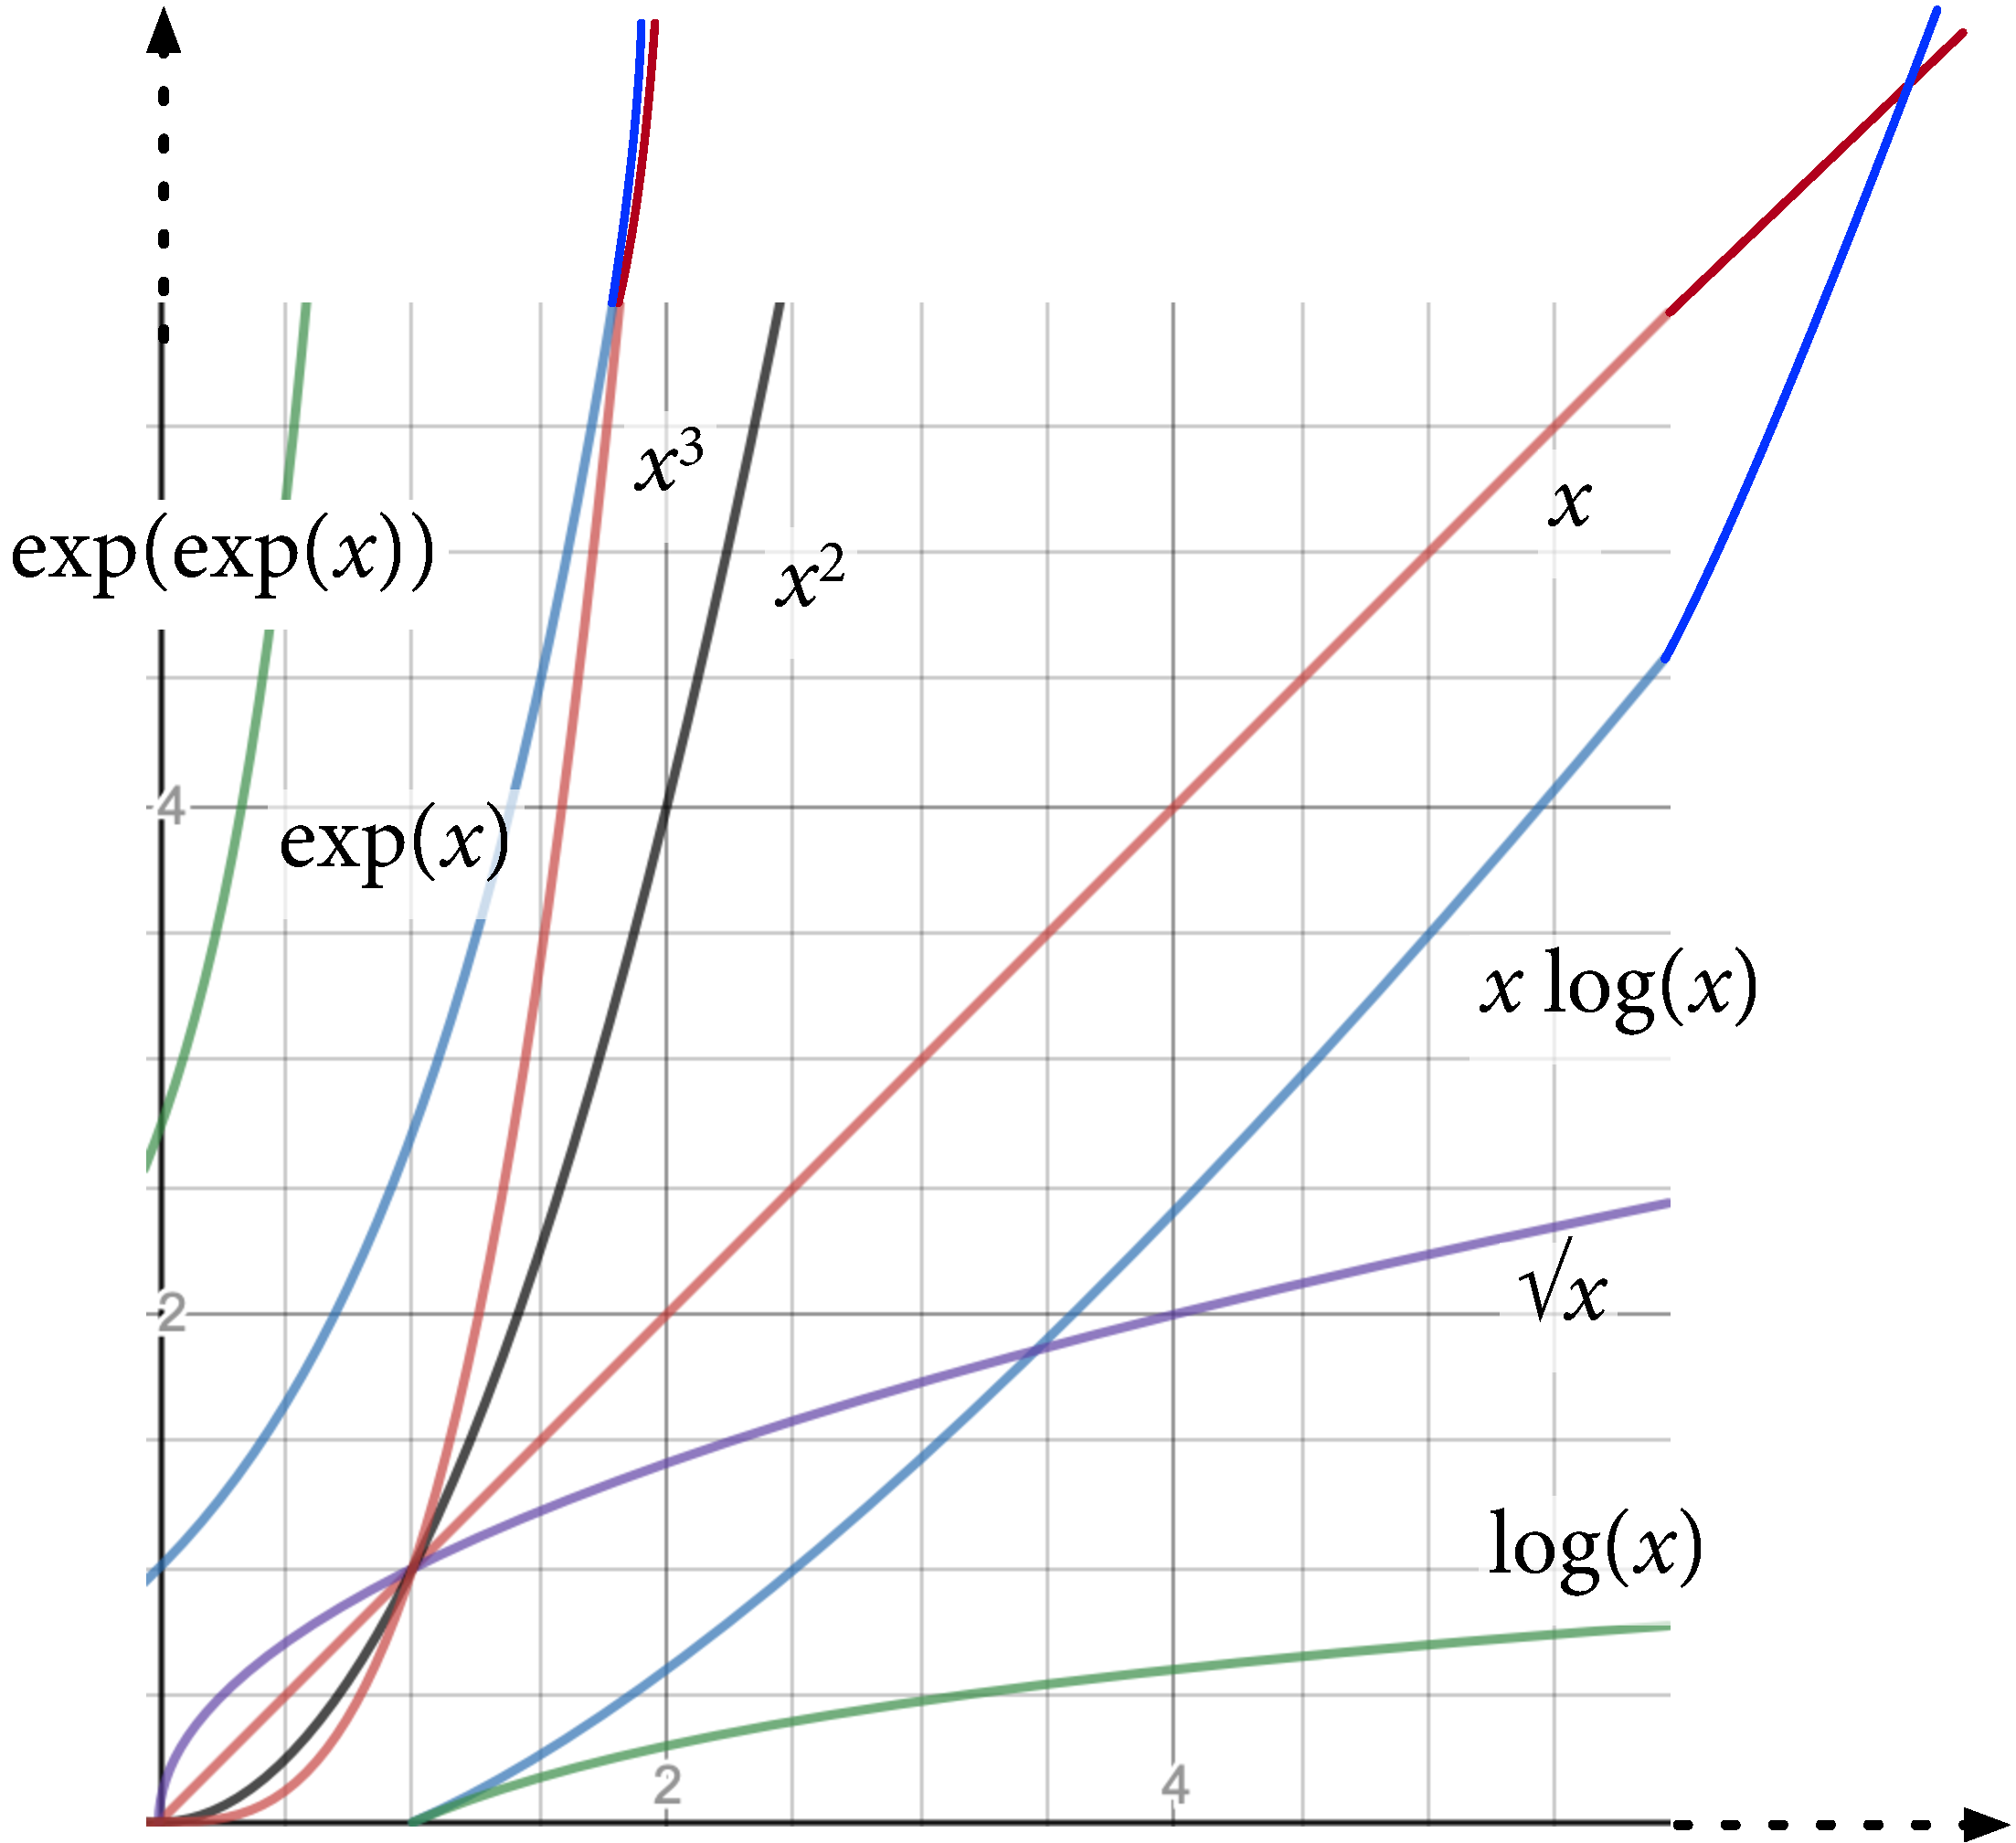
\includegraphics[width=10cm]{pic/GrowthOrders.pdf}
\end{center}
\caption{Some common growth functions}
\label{figcomcl}
\end{figure}
The most prominent class distinctions are sub-linear, linear, polynomial and
exponential+beyond, since the composition of functions in these classes
(which corresponds one algorithm calling another one)
again lies in the same class.

